\documentclass{article}
\usepackage{amsmath, fullpage}
\usepackage[portuguese]{babel}
\usepackage{graphicx}
\usepackage{color}
\usepackage[normalem]{ulem}
\newcommand{\uvec}[1]{\boldsymbol{\hat{\textit{#1}}}}
\graphicspath{{image/}}
\newcommand{\stkout}[1]{\ifmmode\text{\sout{\ensuremath{#1}}}\else\sout{#1}\fi}
\begin{document}
\title{Introdução à mecanica dos fluidos \\ Fenômenos de transporte}
\author{Henrique Bernardes}
%\date{\vspace{-5ex}}
\maketitle \thispagestyle{empty}

\section{Início}
Começamos com a ideia de um pequeno elemento estacionário de fluido em uma certa posição arbitrária de massa do fluido como visto em \ref{fig:forcasuperficieecampo}. Também, sabemos que existem dois tipos de forças que atuam sobre esse elemento:
\begin{itemize}
     \item forças de superfície \( \rightarrow \) devidas à pressão
     \item força de campo \( \rightarrow \) igual ao peso do elemento(no caso estudado, igual a força gravitacional)
\end{itemize}

O peso \( \delta W\) (ou \( d\vec{F_g}\)) atua no sentido negativo da direção z e pode ser descrito como:
 \begin{equation}
      \delta W = \vec{g}*dM 
 \end{equation}
mas como sabemos da fórmula de massa específica, \( dM = \rho dV \), onde \( dV= dxdydz\), a equação se torna:
\begin{equation}
     \delta W = \vec{g} \rho  \delta x \delta y \delta z
\end{equation}
Por fim, \( \gamma = \rho \vec{g}\), assim,

\begin{equation}
     \delta W = \gamma  \delta x \delta y \delta z
\end{equation}


\begin{figure}[!h]
     \centering
     \def\svgwidth{0.4\textwidth}
     \input{image/inomeado.eps_tex}
     \caption{\label{fig:forcasuperficieecampo} Forças de superfície e campo atuando em um pequeno elemento de fluido.}
     \hfill
\end{figure}
 

Sabemos que a soma das forças sobre esse elemento de volume d\sout{V} deve ser 0 para atender à condição de equilíbrio, ou seja

\begin{equation}
     d\vec{F}=d\vec{F_g}+d\vec{F_p}
     \label{equacaoGeral}
\end{equation}

Já deduzimos que as forças de campo se resumem à:

\begin{equation}
     d\vec{F_g}=dM*\vec{g}=\rho \vec{g} dxdydz
\end{equation}

Agora, para as forças de superfície, temos o seguinte:

\begin{equation}
     d\vec{F_p}=P(x,y,z)A
\end{equation}

Considerando a componente x e expandindo em Taylor:
\begin{align*}
d\vec{F_{px}} &= [P(x,y,z)-P(x+dx,y,z)]dydz \rightarrow  P(x+dx,y,z)=P(x,y,z)+\frac{\partial P}{\partial x}dx+...\\ 
&= \left[P(x,y,z)-P(x,y,z)-\frac{\partial P}{\partial x}dx\right]dydz\\
&= -\frac{\partial P}{\partial x}dxdydz\ .
\end{align*}
Então: 
\begin{equation}
    d\vec{F_{px}}= -\frac{\partial P}{\partial x}dxdydz\ .
\end{equation}
Para os outros componentes:
\begin{align}
d\vec{F_{py}}= -\frac{\partial P}{\partial y}dxdydz \\    
d\vec{F_{pz}}= -\frac{\partial P}{\partial z}dxdydz \
\end{align}

Assim sendo, temos o o seguinte:

\begin{equation}
     \sum{d\vec{F_p}} = \underbrace{-\left(\frac{\partial P\uvec{i}}{\partial x} + \frac{\partial P\uvec{j}}{\partial y} + \frac{\partial P\uvec{k}}{\partial z}\right)}_{\vec{\nabla} P}dxdydz
\end{equation}
Onde $d\vec{F_p}$ é um campo vetorial de força associado ao campo escalar de pressão.

Ou seja:

\begin{equation}
     \sum{d\vec{F_p}}=-\vec{\nabla}Pdxdydz 
\end{equation}

Substituindo os valores de $d\vec{F_p}$ e $d\vec{F_g}$ na equação \ref{equacaoGeral}, obtemos:

\begin{align*}
&d\vec{F_g} + d\vec{F_p}=0\\
&\rho \vec{g}dxdydz - \vec{\nabla}Pdxdydz=0\\
&(-\vec{\nabla}P + \rho\vec{g}) dxdydz=0\\
&(\underbrace{-\vec{\nabla}P}_a + \underbrace{\rho\vec{g}}_b)=0\
\end{align*}
O termo \textit{a} indica a força de pressão resultante por unidade de volume em um ponto. Já o termo \textit{b} indica a força de campo por unidade de volume em um ponto.
\newpage
Decompondo nas direções x, y, e z:

\begin{align}
-\frac{\partial P}{\partial x} + \rho \vec{g}=&0\\
-\frac{\partial P}{\partial y} + \rho \vec{g}=&0\\
-\frac{\partial P}{\partial z} + \rho \vec{g}=&0\
\end{align}

Escolhendo o eixo z para cima:
\begin{figure}[!h]
     \centering
     \def\svgwidth{0.25\textwidth}
     \input{image/gCord.eps_tex}
     \caption{\label{fig:gravidadeCoordenadas} Eixo de coordenadas com vetor $\vec{g}$ indicado.}
     \hfill
\end{figure}

vemos então que:
\begin{align*}
\frac{\partial P}{\partial x}=0 ;\ 
\frac{\partial P}{\partial y}=0 ;\
\frac{\partial P}{\partial z} = -\rho \vec{g}\
\end{align*}

Assim sendo, como $P$ é uma função de uma só variável, a derivada parcial pode ser substituida pela derivada total:
\begin{equation}
     \frac{dP}{dz}=-\rho \vec{g}
     \label{equacaoFinalDerivada}
\end{equation}

Isto é, assumindo as seguintes premissas:
\begin{enumerate}
     \item O fluido é estatico;
     \item A gravidade é a única força de campo;
     \item O eixo z é vertical para cima.
\end{enumerate}

 
Para um líquido incompressível, $\gamma = cte$, ou seja, $\rho = cte$ e $g = cte$. Assim sendo, manipulando e integrando a equação \ref{equacaoFinalDerivada}, aplicando as condições de contorno, onde consideramos a pressão no nível de referência (z0) como sendo $P_0$, então a pressão P no nível z é dada por:

\begin{align*}
\frac{dP}{dz} &=-\rho g \\
dP &= -\rho g dz\\
\int_{P_0}^{P} \,dP &= -\rho g \int_{z_0}^{z}\,dz \\
P-P_0 &= -\rho g (z-z_0) \\
\end{align*}

\begin{equation}
\boxed{P-P_0 = +\rho g (z_0-z)}     
\label{eqFinal}
\end{equation}

Como visto na equação \ref{eqFinal}, a pressão em um líquido incompressível em repouso depende da altura h($h=z_0-z$) do fluido em relação a um plano de referência e \textbf{não} é influenciada pelo tamanho ou forma do tanque no qual o fluido se encontre. Também, a equação \ref{eqFinal} só é válida para fluidos na qual o peso específico $\gamma$ é constante. Para aqueles na qual $\gamma$ não é constante, a forma como varia deve ser especificada antes que a equação \ref{equacaoFinalDerivada} possa ser integrada.



\subsection{Exercicio 11.1}
Vamos calcular a pressão \textbf{manométrica}(ou seja, em relação à pressão atmosférica) na interface gasolina-água e na parte inferior do tanque em $\frac{lbf}{in^2}$ e a altura de carga da coluna de água em $ft$:
\begin{figure}[!h]
     \centering
     \def\svgwidth{0.5\textwidth}
     \input{image/exercicio11_1.eps_tex}
     \caption{\label{fig:exercicio11_1} Exercicio 11.1}
     \hfill
\end{figure}
Primeiro, calculamos a pressão no ponto 1, indo do ponto 0 ao ponto 1, tendo $\gamma_{gasolina}=42.5 \frac{lbf}{ft^3}$ e $\gamma_{agua}=62.4 \frac{lbf}{ft^3}$:

\begin{align*}
p_1 - p_0 &= \gamma_{gasolina}h_{1\rightarrow0}\\     
p_1 - p_0 &= \gamma_{gasolina}h_{1\rightarrow0}\\
p_1 - p_0 &= 42.5 \frac{lbf}{ft^3} * 17ft \\ 
p_1 - p_0 &= 722.5 \frac{lbf}{ft^2} \left|\frac{1ft^2}{144 in^2} \right| \\
p_1 - p_0 &= 5.02 \frac{lbf}{in^2}\\
\end{align*}

Tendo o valor da pressão no ponto intermediario em relação ao ponto 0, podemos calcular a pressão no ponto 2 com relação ao ponto 1(indo do ponto 1 ao ponto 2):

\begin{align*}
p_2 - p_1 &= \gamma_{agua}h_{2\rightarrow1} \\
p_2 &= \gamma_{agua}h_{2\rightarrow1} + p_1\\
p_2 &= 62.4 \frac{lbf}{ft^3} * 3ft + 722.5 \frac{lbf}{ft^2} + p_0\\
p_2 - p_0 &= 909.7 \frac{lbf}{ft^2} \left| \frac{1ft^2}{144in^2} \right| \\
p_2 - p_0 &= 6.32 \frac{lbf}{in^2}\\
\end{align*}

Assim sendo, calculamos a altura de carga da coluna de água:
\begin{align*}
h_{0\rightarrow2}&=\frac{p_2-p_0}{\gamma_{agua}}\\
h_{0\rightarrow2}&=\frac{6.32 lbf/in^2}{62.4 lbf/ft^3}\\
h_{0\rightarrow2}&=\frac{0.10 ft^3}{in^2} \left| \frac{144in^2}{ft^2} \right|\\ 
h_{0\rightarrow2}&=14.58ft
\end{align*}

\subsection{Medições de pressão}

A pressão em um ponto interior de uma massa de fluido pode ser designada ou por \textbf{pressão absoluta} ou por \textbf{pressão manométrica}. A pressão absoluta é a medida em relação à pressão zero absoluta, enquanto a pressão manométrica é medida em relação à pressão atmosférica local.

Pressões absolutas são sempre positivas, mas a pressão manométrica pode ser ou positiva ou negativa, a depender se a pressão está abaixo ou acima da pressão atmosférica. Uma pressão manométrica negativa é também chamada de pressão de vácuo. Por exemplo, uma pressão absoluta de 10psi poderia ser representada como uma pressão manométrica de -4.7psi se a pressão atmosférica local fosse 14.7psi, ou então como 4.7 psi de sucção/vácuo. 

Para a maioria  das análises de mecânica dos fluidos é prática usual utilizar a pressão manométrica.

\subsection{Manômetros}
São dispositivos de medição de pressão que envolvem o uso de colunas de líquidos em tubos verticais ou inclinados. 
\subsubsection{Tubo Piezométrico}
Consiste em um tubo vertical, aberto na parte superior e fixado a um recipiente cuja pressão se deseja determinar.

\begin{figure}[!h]
     \centering
     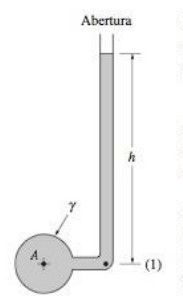
\includegraphics[width=0.2\textwidth]{tuboPiezometrico.jpg} 
     \caption{Tubo Piezometrico}
     \label{fig:tuboPiezometrico} 
     \hfill
\end{figure}

Uma vez que os manômetros envolvem colunas de fluidos em repouso, a equação fundamental que descreve seu uso é $p=\gamma h + p_0$, fornecendo a pressão em qualquer elevação no interior de um fluido homogêneo em termos da pressão de referência $p_0$ e da distância h entre $p$ e $p_0$. É importante mencionar que, uma vez que o tubo é aberto na parte superior, a pressão manométrica $p_0=0$, dado que:
\begin{align*}
p_{manometrica}&=p_{absoluta}-p_{atmosferica}\\
p_{manometrica}&=p_{atmosferica}-p_{atmosferica}\\
p_{manometrica}&=0
\end{align*}

Logo, a equação fundamental se reduz à:
\begin{align*}
     p = p_A = \gamma h 
\end{align*}

Embora o tubo piezométrico seja simples e preciso, apresenta algumas desvantagens:
\begin{enumerate}
     \item Só é apropriado se a pressão no recipiente for maior do que a pressão atmosférica(caso contrário, o ar seria sugado pelo sistema.);
     \item Só é apropriado se a pressão a ser medida for relativamente baixo, de modo que a altura necessária da coluna não seja muito elevada;
     \item O fluido no interior do recipiente cuja pressão deverá ser medida deverá ser um líquido e não um gás.
\end{enumerate}

\subsubsection{Manômetro de tubo em U}
Visando superar as dificuldades observadas no tubo piezométrico, utiliza-se o manômetro de tubo em U. O fluido no manômetro é chamado de \textbf{fluido manométrico}. Para determinar a pressão $p_A$ em termos das variações das alturas das colunas, começamos em uma extremidade do sistema e seguimos até a outra extremidade, utilizando apenas a equação fundamental.

\begin{figure}[h]
     \centering
     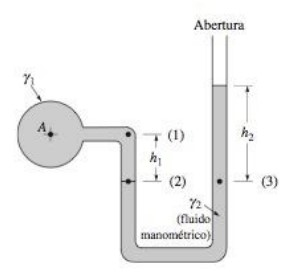
\includegraphics[width=0.3\textwidth]{manometroemtubosimples.jpg} 
     \caption{Manômetro em U simples} 
     \label{fig:manometroemtubosimples} 
     \hfill
\end{figure}



No caso da figura \ref{fig:manometroemtubosimples}, começamos na extremidade aberta seguindo para o ponto A($p-p_0 \rightarrow p_A-0$)\footnote{Vale a explicação mais detalhada: inicialmente, temos $p-p_0 = \gamma h$, onde $p$ é a pressão final e $p_0$ é a pressão inicial. Assim sendo, para determinar a diferença de pressão entre o ponto A e o ponto B, começamos no ponto A and terminamos no ponto B, ou seja, $p_B - p_A$. Poderiamos, alternativamente, determinar a diferença de pressão entre o ponto B e o ponto A, começando no ponto B e terminando no ponto A, ou seja, $p_A - p_B$. Segue a recomendação de \textbf{SEMPRE} seguir o caminho \textbf{ATÉ} o ponto onde se deseja conhecer a pressão. Logo, na figura \ref{fig:manometroemtubosimples}, começamos no ponto aberto e vamos para o ponto A, a equação se torna, então, $p_A-p_0$. Já na figura \ref{fig:manometroemtubodiferencial}, independe a ordem, mas, como indicado pela forma como foi fornecida a equação final no livro, devemos ir do ponto B até o ponto A, ou seja, $p_A - p_B$.} A pressão no ponto A e (1) são as mesmas e à medida que vamos do ponto (1) para o (2) a pressão aumentará em $\gamma_1 h_1$. A pressão no ponto (2) é igual à pressão no ponto 3, uma vez que as pressões em elevações iguais em uma massa contínua de fluido em repouso devem ser as mesmas(observe que não é possível "pular" do ponto (1) para um ponto de mesma elevação ao outro lado do tupo pois podem ser pontos de massa contínua de fluido diferentes). Com a pressão em (3) especificada, movemos para a extremidade aberta onde a pressão manométrica é 0. Como nos movemos para cima, a pressão decresce em magnitude $\gamma_2 h_2$. Em forma de equação:
\begin{align*}
\boxed{p_1-p_0 = p_A = \gamma_2 h_2 - \gamma_1 h_1}
\end{align*}

Uma das vantagens do manômetro de tubo em U está no fato que o fluido manométrico pode ser diferente do fluido no recipiente cuja pressão deve ser determinada. Por exemplo, o fluido em (A), (ainda na figura \ref{fig:manometroemtubosimples}) pode ser um líquido ou um gás. Se A contiver um gás, a contribuição da coluna de gás $\gamma_1 h_1$ é quase sempre desprezível de modo que $p_A=p_2$, ou seja, 
\begin{align*}
p_A=\gamma_2 h_2
\end{align*}

O peso específico $\gamma$, de um líquido, como fluido manométrico, é frequentemente representado em termos da densidade $D$, pela razão:

\begin{align}
     \gamma = D\gamma_{agua} = Dg\rho_{agua}
\end{align}
Um manômetro em U pode também ser utilizado para determinar a diferença na pressão entre dois recipientes, como na figura \ref{fig:manometroemtubodiferencial}

\begin{figure}[!h]
     \centering 
     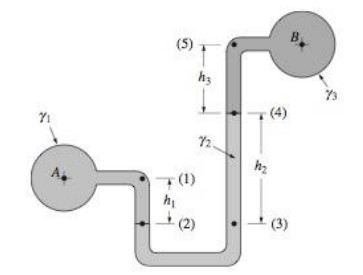
\includegraphics[width=0.3\textwidth]{manometroemtubodiferencial.jpg} 
     \caption{Manômetro em U diferencial} 
     \label{fig:manometroemtubodiferencial} 
\end{figure}
Para determinar diferença na pressão entre A e B começamos novamente em uma extremidade do sistema e seguimos até a outra.

A pressão em A($p_A$) é igual à pressão em (1), ou seja, $p_A = p_1$ e, a medida que nos deslocamos para o ponto (2), a pressão aumenta em $\gamma_1 h_1$. A pressão em (2) é igual à pressão em (3), ou seja $p_2 = p_3$ e, a medida que nos deslocamos para (4), a pressão diminui em $\gamma_2 h_2$. De forma similar, a medida que nos deslocamos de (4) para (5), a pressão diminui em $\gamma_3 h_3$. Por fim, temos que a pressão em (B) é igual à pressão em (5), ou seja, $p_B=p_3$. Em forma de equação:
\begin{align*}
\boxed{p_A-p_B=\gamma_3 h_3 + \gamma_2 h_2 - \gamma_1 h_1}
\end{align*}
\newpage
\subsection{Exercício 11.8} 

\begin{figure}[!h]
     \centering
     \def\svgwidth{0.8\textwidth}
     \input{image/exercicio11_8.eps_tex}
     \caption{\label{fig:exercicio11.8} Exercicio 11.8}
     \hfill
\end{figure}

Neste exercício, devemos determinar algumas coisas:
\begin{enumerate}
     \item A altura h
     \item A pressão manométrica na superfício AB
     \item A pressão absoluta do ar no topo do tanque se a pressão atmosférica local é de 14.7 psi absoluta.
\end{enumerate}

Para determinarmos a altura h, naturalmente vamos precisar saber a pressão em (3), uma vez que:
\begin{align*}
     p_4-p_3&=-\gamma_{agua}h\\
     p_3&=\gamma_{agua}h\\
     \frac{p_3}{\gamma_{agua}}&=h
\end{align*}
uma vez que $p_4=0$(a pressão absoluta se iguala a pressão atmosférica, logo a pressão monométrica é zero).
Assim sendo, para determinarmos a pressão em (3), basta determinarmos a pressão em (2), pois estão no mesmo nível.
Determinando a pressão em (2):
\begin{align*}
     p_2-p_1&=\gamma_{agua}h_{2\rightarrow1}\\
     p_2&=\gamma_{agua}h_{2\rightarrow1}+p_1\\
     p_2&=62.4\frac{lbf}{ft^3}\left|\frac{1ft^2}{144in^2}\right|2ft+7\frac{lbf}{in^2}\\
     p_2&=7.86\frac{lbf}{in^2}
\end{align*}
\newpage
Feito isso, podemos 1) dizer que $p_3=p_2$ e substituir na fórmula de p3, ou 2) igualar ambas as fórmulas de p2 e p3, ou seja, respectivamente:

\begin{figure}[!h]
\centering
\begin{minipage}{0.5\textwidth}
     1)
     \begin{align*}
     p_3&=\gamma_{agua}*h\\
     \frac{7.86lbf}{in^2}&=62.4\frac{lbf}{in^2}*h\\
     \frac{7.86lbf/in^2}{62.4lbf/in^2}&=h\\
     18.13ft&=h
\end{align*}
\end{minipage}\hfill
\begin{minipage}{0.5\textwidth}
     2)
   \begin{align*}
     p_2&=p_3\\
     \frac{7.86lbf}{in^2}&=62.4\frac{lbf}{in^2}*h\\
     \frac{7.86lbf/in^2}{62.4lbf/in^2}&=h\\
     18.13ft&=h
\end{align*}
\end{minipage}
\end{figure}

Naturalmente, ambas levam ao exato mesmo lugar, somente foi destacado como forma de desenvolvimento de intuição no contexto destes problemas.
 

Para determinar a pressão manométrica na superfície AB, também temos duas opções. Podemos 1) utilizar o valor já calculado de $p_2$ e "caminhar" de (2) até (5), ou 2) ir de (1) até (5) considerando novamente a pressão manométrica medida de 7psi, respectivamente:

\begin{figure}[!h]
\centering
\begin{minipage}{0.5\textwidth}
     1)
     \begin{align*}
          p_5-p_2&=\gamma_{agua}h_{5\rightarrow2}\\
          p_5&=\gamma_{agua}h_{5\rightarrow2}+p_2\\
          p_5&= 62.4\frac{lbf}{ft^3} \left|\frac{1ft^2}{144in^2} \right|2ft+7.86\frac{lbf}{in^2}\\
          p_5&=8.73\frac{lbf}{in^2}
     \end{align*}
\end{minipage}\hfill
\begin{minipage}{0.5\textwidth}
     2)
     \begin{align*}
          p_5-p_1&=\gamma_{agua}h_{5\rightarrow1}\\
          p_5&=\gamma_{agua}h_{5\rightarrow1}+p_1\\
          p_5&=62.4\frac{lbf}{ft^3}\left|\frac{1ft^2}{144in^2} \right|4ft+7\frac{lbf}{in^2}\\
          p_5&=8.73\frac{lbf}{in^2}
     \end{align*}
\end{minipage}
\end{figure}

Finalmente, devemos determinar a pressão absoluta do ar no topo do tanque tendo o valor da pressão atmosférica local de 14.7 psi. Sabemos que $p_{monometrica}=p_{absoluta}-p_{atmosferica}$, logo, basta substituir os valores na fórmula:

\begin{align*}
     p_{monometrica}&=p_{absoluta}-p_{atmosferica}\\
     p_{monometrica}+p_{atmosferica}&=p_{absoluta}\\
     7psi+14.7psi&=p_{absoluta}\\
     21.7psi&=p_{absoluta}\\
\end{align*}

\newpage
\subsection{Exercício de sala}

\begin{figure}[!h]
     \centering
     \def\svgwidth{0.4\textwidth}
     \input{image/exercicioSala.eps_tex}
     \caption{\label{fig:exercicioSala} Exercicio de sala.}
     \hfill
\end{figure}
Primeiramente, queremos descobrir uma fórmula geral para L. Começamos com a fórmula da pressão em (1):
\begin{align*}
     p_1-p_0=\gamma h_1
\end{align*}
Para o ponto (a), sabemos que $p_a=p_0$, logo temos:
\begin{align*}
     p_a-p_1&=-\gamma h_1\\
     p_0-p_1&=-\gamma h_1\\
     p_0&=-\gamma h_1+p_1\\
\end{align*}
Para o ponto (2), temos que:
\begin{align*}
     p_2-p_a&=-\gamma h_2\\
     p_2-p_0&=-\gamma h_2\\
     p_2&=-\gamma h_2+p_0\\
\end{align*}
Substituindo $p_0$ na fórmula de $p_2$:
\begin{align*}
     p_2&=-\gamma h_2+p_0\\
     p_2&=-\gamma h_2+(-\gamma h_1+p_1)\\  
     p_2&=-\gamma h_2-\gamma h_1+p_1\\           
     p_2-p_1&=-\gamma h_2-\gamma h_1\\
     p_1-p_2&=\gamma(h_2+h_1)\\
\end{align*}
Podemos então encontrar o valor de $h_2$:
\begin{align*}
     sin\theta&=\frac{h_2}{L}\\
     h_2&=sin\theta L\\
\end{align*}
Substituindo na fórmula encontrada anteriormente:
\begin{align*}
     p_1-p_2=\gamma(sin\theta L + h_1)\\
\end{align*}
Para acharmos $h_1$, devemos introduzir o fato de que o volume de líquido do manômetro permanece constante, logo, o volume deslocado do resertavório deve ser igual ao volume que sobe na coluna, ou seja:
\begin{align*}
     \pi \frac{D^2}{4}h_1&=\pi \frac{d^2}{4}L\\
     h_1&=\frac{d^2}{D^2}L
\end{align*}
Substituindo de volta na fórmula:
\begin{align*}
     p_1-p_2&=\gamma\left(sin\theta L + \frac{d^2}{D^2}L\right)\\
     p_1-p_2&=\gamma L\left(sin\theta + \frac{d^2}{D^2}\right)\\
     L&=\frac{p_1-p_2}{\gamma\left(sin\theta + \frac{d^2}{D^2}\right)}\\
\end{align*}


\subsection{Força Hidrostática Sobre uma Superfície Plana}
Quando uma superfície está submersa em um fluido, são desenvolvidas forças na superfície devidas ao fluido. Note que, nos fluidos em repouso, a força deve ser \textbf{perpendicular} à superfície. 
\subsection{Superfície Plana Horizontal}
\begin{figure}[h]
  \centering
  \begin{minipage}{0.45\textwidth}
    \centering
    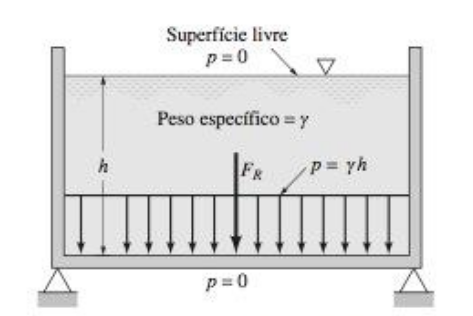
\includegraphics[width=0.8\linewidth]{forcaResultanteSuperficieLivreReta.png}
    \caption{Pressão no fundo de um tanque aberto horizontal}
    \label{fig:forcaResultanteSuperficieLivreReta}
  \end{minipage}\hfill
  \begin{minipage}{0.45\textwidth}
    \centering
    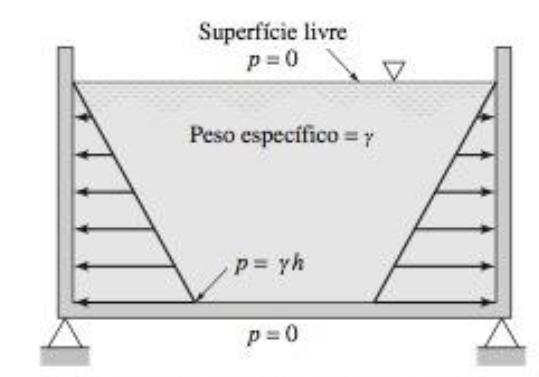
\includegraphics[width=0.8\linewidth]{forcaResultanteSuperficiePlanaParedes.png}
    \caption{Pressão no fundo de um tanque aberto horizontal}
    \label{fig:forcaResultanteSuperficieLivreRetaParedes}
  \end{minipage}
\end{figure}

Para o caso mais simples de uma superfície plana horizontal, como a superfície inferior do tanque aberto da figura \ref{fig:forcaResultanteSuperficieLivreReta}, fica claro que a magnitude da força resultante é simplesmente $F_R=pA$, uma vez que pressão p é uniforme ao longo de toda a superfície, sendo $p= \gamma h$. Uma vez que a pressão é constante e uniformemente distribuida ao longo da superfície inferior, a força resultante atua através do centróide da figura.\footnote{Vale mencionar que a pressão \textbf{NÃO} é uniforme ao longo das paredes verticais do tanque, como na figura \ref{fig:forcaResultanteSuperficieLivreRetaParedes}}
\newpage
\subsection{Superfície Plana Inclinada}
Para o caso mais geral no qual se tem uma superfície plana inclinada submersa, como na figura \ref{fig:forcaResultanteSuperficieInclinada} a determinação da força resultante que atua sobre a superfície é mais complexa, dado que a pressão \textbf{não} será uniforme ao longo da superfície.
\begin{figure}[!h]
  \centering
  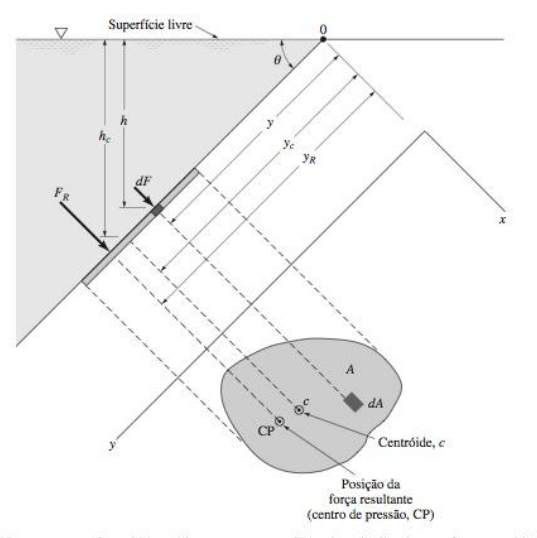
\includegraphics[width=0.6\linewidth]{forcaResultanteSuperficieInclinada.png}
  \caption{Força resultante em uma superfície plana inclinada submersa}
  \label{fig:forcaResultanteSuperficieInclinada}
\end{figure}

Admitimos, inicialmente, que a superfície é aberta à atmosfera. Consideramos o plano no qual a superfície em repouso intercepta a superfície livre em 0, formando um ângulo $\theta$. O sistema de coordenadas x-y é definido de modo que 0 seja a origem e y seja orientado ao longo da superfície. A área pode ter um formado arbitrário. Desejamos determinar a direção, o sentido, a localização e a magnitude da força resultante atuando em um lado dessa área devida ao líquido em contato com a área.

Em uma profundidade fornecida h, a força que atua em dA é $dF = \gamma h dA$ e, como esperado, é perpendicular à superfície. Assim sendo, a intensidade da força resultante pode ser encontrada somando-se essas forças diferenciais em toda a superfície, ou seja:

\begin{equation}
  F_R = \int_{A}^{ } \gamma h\, dA = \int_{A}^{ } \gamma y sin\theta\, dA
  \label{eq:integrandoForcaSuperficieInclinada}
\end{equation}
tendo em vista que:
\begin{align}
  sin\theta &= \frac{h}{y}\\
  h &= y sin\theta \\
  \label{eq:formulaProfundidadeAreaSuperficieInclinada}
\end{align}
Para y e $\theta$ constantes, temos:
\begin{equation}
  F_R=\gamma sin \theta \int_{A}^{ } y\, dA
  \label{eq:forcaResultanteSuperficieInclinada2}
\end{equation}

A integral da equação \ref{eq:forcaResultanteSuperficieInclinada2} é o momento estático(ou primeiro momento) da área em relação ao eixo x e pode ser representado como:
\begin{align}
  \int_{A}^{ } y\, dA = y_cA
\end{align}
onde $y_c$ é a coordenada y do centróide medida a partir do eixo x, que passa por 0.
Podemos, então, reescrever a equação \ref{eq:forcaResultanteSuperficieInclinada2} como:
\begin{align*}
   F_R=\gamma sin\theta y_c A
\end{align*}
Sabendo, também, que $h_c$(altura do eixo x até o centróide da superfície) é dado por:
\begin{align*}
  sin\theta &=\frac{h_c}{y_c} \\
  h_c&=y_c sin\theta 
\end{align*}
logo, a equação se torna:
\begin{equation}
  F_R=\gamma A h_c
  \label{eq:forcaResultanteSuperficieInclinada3}
\end{equation}
Devemos observar que a magnitude da força é independente do ângulo $\theta$ e depende apenas do peso específico do fluido, da área total da superfície plana e da profundidade do centróide da área abaixo da superfície. A equação \ref{eq:forcaResultanteSuperficieInclinada3} indica que a magnitude da força resultante é igual à pressão no centróide da área multiplicada área total.

Embora a nossa intuição possa sugerir que a força resultante deveria passar pelo centróide da área, não é o que de fato ocorre. O ponto através da qual a força resultante atua é chamado de \textbf{centro de pressão} e sua posição em relação ao centróide da área está indicado na figura \ref{fig:centroDePressoaInclinado}.

\begin{figure}[!h]
  \centering
  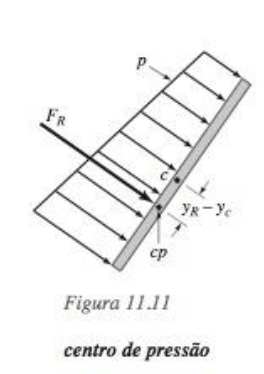
\includegraphics[width=0.3\linewidth]{centroDePressoaInclinado.png}
  \caption{Localização da força resultante e representação da não uniformidade da pressão para uma superfície inclinada em um fluido}
  \label{fig:centroDePressoaInclinado}
\end{figure}

A coordenada $y_R$ da força resultante pode ser determinada pela soma dos momentos em torno do eixo x. Ou seja, o momento da força resultante deve ser igual ao momento da força de pressão distribuida:

\begin{equation}
  F_Ry_R = \int_{A}^{ } y\, dF = \int_{A}^{ } y\gamma h\, dA =\int_{A}^{ } \gamma sen\theta y^2\, dA 
  \label{eq:EqMomentoForcaResultanteIgualMomentoForcaPressao}
\end{equation}
onde $dF=pdA =\gamma h dA$ junto com a fórmula \ref{eq:formulaProfundidadeAreaSuperficieInclinada}, 

É possível demonstrar(?!!?!???!!!!) que essa relação de momentos leva à seguinte equação que fornece a distância $y_r-y_c$ entre o centro de pressão e o centróide:
\begin{equation}
  y_r - y_c = \frac{I_{xc}}{y_cA} 
  \label{eq:equacaoDistanciaCentroPressaoECentroide}
\end{equation}
onde a grandeza $I_{xc}$ denominada momento de inércia(ou segundo momento) da área plana A em relação a um eixo que passa através do centróide A é uma propriedade geométrica da área A, como por exemplo:
\begin{figure}[!h]
  \centering
  \begin{minipage}{0.45\textwidth}
    \centering
    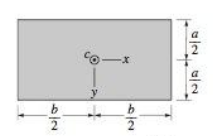
\includegraphics[width=0.7\linewidth]{propriedadesGeometricaRetangulo.png}
    \caption{Propriedades geométricas de um retângulo}
  \end{minipage}\hfill
  \begin{minipage}{0.45\textwidth}
    \centering
    \begin{align*}
      A&=b*a\\
      I_{xc}&=\frac{1}{12}ba^3
    \end{align*}
  \end{minipage}
\end{figure}

\begin{figure}[!h]
  \centering
  \begin{minipage}{0.45\textwidth}
    \centering
    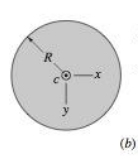
\includegraphics[width=0.7\linewidth]{propriedadesGeometricaCirculo.png}
    \caption{Propriedades geométricas de um circulo}
  \end{minipage}\hfill
  \begin{minipage}{0.45\textwidth}
    \centering
    \begin{align*}
      A&=\pi R^2\\
      I_{xc}&=\frac{\pi R^4}{4}
    \end{align*}
  \end{minipage}
\end{figure}
Finalmente, uma vez que $\frac{I_{xc}}{y_cA}>0$, a equação \ref{eq:equacaoDistanciaCentroPressaoECentroide} mostra que o centro de pressão está \textbf{SEMPRE} abaixo do centróide. 
\newpage
\section{Fluidos em movimento}
As leis básicas que serão aplicadas aqui são:
\begin{enumerate}
  \item A conservação de massa;
  \item A segunda lei de Newton;
  \item O princípio da quantidade de movimento angular;
  \item A primeira e segunda leis de termodinâmica.
\end{enumerate}
Para converter estas equações em fórmulas equivalentes para um volume de controle, vamos expressar cada uma delas como uma equação de taxa.
\subsection{Conservação de Massa}
Para um sistema, sendo por definição uma quantidade de matéria fixa \textit{M}, temos que $M=cte$. Contudo, como já dito, queremos expressar cada lei como uma equação de taxa, logo:
\begin{equation}
  \left.\frac{dM}{dT}\right)_{sistema} = 0
  \label{eq:conservacaoDeMassa}
\end{equation}
em que:
\begin{equation}
  M_{sistema}=\int_{M(sistema)}^{ } \, dm = \int_{\stkout{V}(sistema)}^{ } \rho\, d\stkout{V}
  \label{eq:massaFormula}
\end{equation}
\subsection{Segunda Lei de Newton}
Para um sistema com movimento relativo a um sistema de referência inercial, a segunda lei de Newton estabelece que a soma de todas as forças externas agindo sobre o sitema é igual à taxa de variação com o tempo da quantidade de movimento linear do sistema:
\begin{equation}
  \vec{F}=\left.\frac{d\vec{P}}{dt}\right)_{sistema}
  \label{eq:segundaLeiNewton}
\end{equation}
onde a quantidade de movimento linear do sistema ($\vec{P}$) é dado por:
\begin{equation}
  \vec{P}_{sistema}=\int_{M(sistema)}^{ } \vec{V}\, dm = \int_{\stkout{V}_{sistema}}^{ } \vec{V} \rho\, d\stkout{V} 
  \label{eq:movimentoLinearFormula}
\end{equation}
\subsection{O princípio da quantidade de movimento angular}
O princípio da quantidade de movimento angular para um sistema estabelece que a taxa de variação da quantidade de movimento angular é igual à soma de todos os torques atuando sobre o sistema:
\begin{equation}
  \vec{T}=\left.\frac{d\vec{H}}{dt}\right)_{sistema}
  \label{eq:TorqueIgualVariacaoMovimentoAngular}
\end{equation}
onde a quantidade de movimento angular do sistema é dada por:
\begin{equation}
  \vec{H}_{sistema}=\int_{M(sistema)}^{ } \vec{r} \times \vec{V}\, dm = \int_{\stkout{V}(sistema)}^{ } \vec{r} \times \vec{V} \rho \, d\stkout{V}
  \label{eq:qntMovimentoAngular}
\end{equation}
O torque pode ser produzido por forças de superfície e de campo(neste caso, a gravidade) e também por eixos que cruzam a fronteira do sistema:
\begin{equation}
  \vec{T}=\vec{r} \times \vec{F}_s + \int_{M(sistema)}^{ } \vec{r} \times \vec{g}\, dm + \vec{T}_{eixo} 
  \label{eq:torque}
\end{equation}
\subsection{A primeira lei da termodinâmica}
A primeira lei da termodinâmica enuncia a conservação de energia para um sistema:
\begin{align*}
  dE=\delta Q - \delta W
\end{align*}
Reescrevendo em forma de taxa:
\begin{equation}
  \dot{Q}-\dot{W}=\left.\frac{dE}{dt}\right)_{sistema}
  \label{eq:1aLeiTermodinamicaTaxa}
\end{equation}
onde a energia total do sistema é dada por:
\begin{equation}
  E_{sistema}=\int_{M(sistema)}^{ } e\, dm = \int_{\stkout{V}(sistema)}^{ } e\rho\, d\stkout{V}
  \label{eq:energiaTotalSistema}
\end{equation}
onde $e$ é dado por
\begin{align*}
  e = u+\frac{V^2}{2}+gz
\end{align*}
onde cada termo diz respeito à energia interna específica, energia cinética e energia potencial, respectivamente. Adicionalmente, na equação \ref{eq:1aLeiTermodinamicaTaxa}, o termo $\dot{Q}$ é positivo quando o sistema recebe calor; já o termo $\dot{W}$ é positivo quando o sistema realiza trabalho sobre sua vizinhança.
\subsection{A segunda lei da termodinâmica}
Se uma quantidade de calor $\delta Q$ for transferida para um sistema a temperatura T, a segunda lei da termodinâmica estabelece que a variação de entropia dS do sistema satisfaz a relação:
\begin{align*}
   dS\ge\frac{\delta Q}{T}
\end{align*}
em forma de taxa:
\begin{equation}
  \left.\frac{dS}{dT}\right)_{sistema}\ge \frac{1}{T}\dot{Q}
  \label{eq:entropiaTaxa}
\end{equation}
onde a entropia total do sistema é dada por:
\begin{equation}
  S_{sistema}=\int_{M(sistema)}^{ } s\, dm=\int_{\stkout{V}(sistema)}^{ } s \rho \, d\stkout{V}
  \label{eq:entropiaTotalSistema}
\end{equation}
Agora, com a cinco leis básicas expressas em forma de taxa para um sistema, podemos desenvolver uma expressão geral para converter uma equação de taxa para um sistema em uma equação equivalente para um volume de controle. Em vez de converter as equações individualmente(equações \ref{eq:conservacaoDeMassa} \ref{eq:segundaLeiNewton} \ref{eq:TorqueIgualVariacaoMovimentoAngular} \ref{eq:1aLeiTermodinamicaTaxa} e \ref{eq:entropiaTaxa} ), representamos todas as variáveis pelo símbolo $N$. Assim sendo, $N$ representa a quantidade de massa, ou quantidade de movimento, ou quantidade de movimento angular, ou energia, ou entropia de um sistema. Correspondendo a esta propriedade extensiva $N$, precisamos também da propriedade intensiva $\eta$. Ou seja:
\begin{equation}
  N_{sistema}=\int_{M(sistema)}^{ } \eta \, dm = \int_{\stkout{V}(sistema)}^{ } \eta \rho\, d\stkout{V}
  \label{eq:equacaoGeralPropExtensivaPropIntensiva}
\end{equation}
Comparando esta equação com as equações \ref{eq:massaFormula} \ref{eq:movimentoLinearFormula} \ref{eq:qntMovimentoAngular} \ref{eq:energiaTotalSistema} e \ref{eq:entropiaTotalSistema}, chegamos as seguintes relações:
\begin{align*}
  \ref{eq:massaFormula}) &N=M, \eta=1\\
  \ref{eq:movimentoLinearFormula}) &N=\vec{P}, \eta=\vec{V}\\
  \ref{eq:qntMovimentoAngular}) &N=\vec{H}, \eta=\vec{r} \times \vec{V}\\
  \ref{eq:energiaTotalSistema}) &N=E, \eta=e \\
  \ref{eq:entropiaTotalSistema}) &N=S, \eta=s \\
\end{align*}
\begin{figure}[!h]
  \centering
  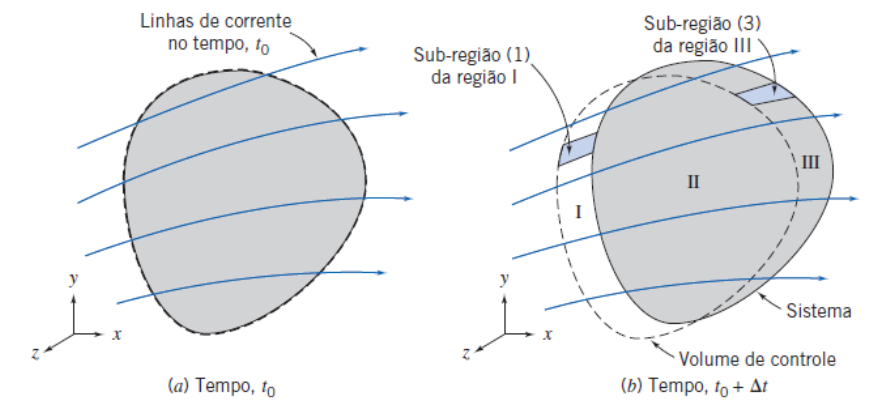
\includegraphics[width=0.8\linewidth]{regioesFluido.png}
  \caption{Configuração para sistema e volume de controle}
  \label{fig:sistemaEVolControle}
\end{figure}
Agora, por meio da análise da figura \ref{fig:sistemaEVolControle} é possível obter a relação fundamental entre a taxa de variação de qualquer propriedade extensiva arbitrária N de um sistema e as variações dessa propriedade associadas a um volume de controle:
\begin{equation}
  \left.\frac{dN}{dt}\right)_{sistema}=\frac{\partial}{\partial t}\int_{VC}^{ } \eta \rho \, d\stkout{V} + \int_{SC}^{ } \eta \rho \vec{V} \cdot \, d\vec{A}
  \label{eq:RelacaoFundamentalReynolds}
\end{equation}
onde $VC$ é o volume de controle e $SC$ é o sistema de controle. O sistema é a matéria que está passando através do volume de controle escolhido no instante escolhido. Se escolhermos, por exemplo, um volume de controle retangular contendo uma asa de uma aeronave, o sistema seria a massa de ar que está instantaneamente contida entre o retângulo e a asa. Na fórmula \ref{eq:RelacaoFundamentalReynolds}, precisamos entender o significado de cada termo:

\begin{figure}[!h]
  \centering
  \begin{minipage}{0.45\textwidth}
    \begin{align*}
      \left.\frac{dN}{dt}\right)_{sistema}
    \end{align*}
  \end{minipage}\hfill
  \begin{minipage}{0.45\textwidth}
    é a taxa de variação da propriedade extensiva do sistema N. Por exemplo, se $N=\vec{P}$, obtemos a taxa de variação da quantidade de movimento.
  \end{minipage}
\end{figure}

\begin{figure}[!h]
  \centering
  \begin{minipage}{0.45\textwidth}
    \begin{align*}
      \frac{\partial}{\partial t} \int_{VC}^{ } \eta \rho \, d\stkout{V}
    \end{align*}
  \end{minipage}\hfill
  \begin{minipage}{0.45\textwidth}
    é a taxa de variação da quantidade da propriedade N dentro do volume de controle. O termo $\int_{VC}^{ } \eta \rho \, d\stkout{V}$  calcula o valor instantâneo de N dentro do volume de controle. Portante, se $N=\vec{P}$, então $\eta = \vec{V}$ e logo $\int_{VC}^{ } \stkout{V} \rho \, d\stkout{V}$ calcula a quantidade de movimento no volume de controle.
  \end{minipage}
\end{figure}

\begin{figure}[!h]
  \centering
  \begin{minipage}{0.45\textwidth}
    \begin{align*}
      \int_{SC}^{ } \eta \rho \vec{V}\ \cdot d\vec{A}
    \end{align*}
  \end{minipage}\hfill
  \begin{minipage}{0.45\textwidth}
    É a taxa na qual a propriedade N está saindo da superficie do volume de controle. O termo calcula o fluxo líquido de N para fora do volume de controle. Então, se $N=\vec{P}$ então $\eta=\vec{V}$ logo $\int_{VC}^{ } \vec{V} \rho \vec{V} \cdot\, d\vec{A}$ calcula o fluxo líquido de quantidade de movimento para fora do volume de controle.
  \end{minipage}
\end{figure}

\subsection{Conservação da massa}
O primeira princípio físico para o qual aplicamos a relação entre as fórmulas de sistema e de volume de controle é o princípio de conservação de massa - a massa do sistema permanece constante:
\begin{align*}
  \left.\frac{dM}{dt}\right)_{sistema}=0
\end{align*}
onde, novamente
\begin{align*}
  M_{sistema}=\int_{M(sistema)}^{ } \, dm = \int_{\stkout{V}(sistema)}^{ } \rho\, d\stkout{V}
\end{align*}

As formulações de sistema e de volume de controle são:

\begin{equation}
  \left.\frac{dM}{dt}\right)_{sistema}=\underbrace{\frac{\partial}{\partial t}\int_{VC}^{ } \rho \, d\stkout{V}}_{\text{1}} + \underbrace{\int_{SC}^{ } \rho \vec{V} \cdot \, d\vec{A}}_{2} = 0
  \label{eq:conservacaoDeMassaFormulacao}
\end{equation}
onde o termo 1 representa a taxa de variação da massa dentro do volume de controle; o termo 2 representa a taxa líquida de fluxo de massa para fora através da superfície de controle.
 Ou seja, a soma da taxa de variação da massa dentro do volume de controle com a taxa líquida de fluxo de massa através da superfície de controle é zero. Essa equação é também chamada de equação da continuidade. Ou seja, a taxa de aumento de massa no volume de controle é decorrente do fluxo líquido de entrada de massa:
\begin{align*}
  \frac{\partial}{\partial t}\int_{VC}^{ } \rho \, d\stkout{V} = -\int_{SC}^{ } \rho \vec{V} \cdot \, d\vec{A}
\end{align*}

Em casos especiais, é possível simplificar a equação \ref{eq:conservacaoDeMassaFormulacao}. Primeiramente, consideramos o caso de um fluido incompressível, onde a massa específica permanece constante. Quando $\rho = cte$ ele não é uma função do espaço e nem do tempo, logo, para fluidos incompressíveis, podemos escrever a equação \ref{eq:conservacaoDeMassaFormulacao} como:
\begin{align*}
  \rho \frac{\partial}{\partial t}\int_{VC}^{ } \, d\stkout{V} + \rho \int_{SC}^{ } \vec{V} \cdot \, d\vec{A}=0
\end{align*}
A integral sobre todo o volume de controle é simplesmente o volume total do volume de controle. Assim, dividindo por $\rho$:
\begin{align*}
 \frac{\partial \stkout V}{\partial t} +  \int_{SC}^{ } \vec{V} \cdot \, d\vec{A}=0
\end{align*}
Para um volume de controle não deformável, de forma e tamanho fixos, $\stkout{V} = cte$. Assim, a conservação de massa para um escoamento incompressível através de um volume de controle fixo torna-se:
\begin{equation}
  \int_{SC}^{ } \vec{V}\cdot\, d\vec{A}=0
  \label{eq:conservacaoMassaEscoamentoIncompressivel}
\end{equation}
Um caso especial útil é quando a velocidade é (ou pode ser aproximada como) uniforme em cada entrada e saída. Aqui, a equação \ref{eq:conservacaoMassaEscoamentoIncompressivel} simplifica-se para:
\begin{equation}
  \sum\nolimits_{SC} \vec{V} \cdot \vec{A}=0
  \label{eq:conservacaoMassaEscoamentoIncompressivelVelocidadeUniforme}
\end{equation}

É interessante notar que em nenhum momento impusemos a restrição de escoamento de regime permanente, somente de escoamento incompressível, assim, a equação \ref{eq:conservacaoMassaEscoamentoIncompressivel} pode ser usada tanto para um escoamento de fluido incompressível em regime transiente ou permanente. As dimensões do integrando são $L^3/t$. A integral sobre uma seção da superfície de controle é chamada de vazão volumétrica(ou taxa de fluxo de volume, ou vazão de volume). Assim sendo, para um escoamento incompressível, a vazão volumétrica para dentro de um volume de controle deve ser igual à vazão volumétrica para fora do volume de controle. Dessa forma, a vazão volumétrica $Q$, através de uma seção de uma superfície de controle de área A é dada por:
\begin{equation}
  Q=\int_{A}^{ } \vec{V}\ \cdot\, d\vec{A}
  \label{eq:vazaoVolumetrica}
\end{equation}
O módulo da velocidade média $\vec{V}$ em uma seção é definido por:
\begin{equation}
    \vec{V}=\frac{Q}{A}=\frac{1}{A}\int_{A}^{ } \vec{V} \cdot\, d\vec{A}
  \label{eq:moduloVelocidadeMedia}
\end{equation}
Considerando o caso de escoamento permanente, compressível através de um volume de controle fixo. Como o escoamento é permanente, no máximo $\rho=\rho(x,y,z)$. Por definição, em regime permanente, nenhuma propriedade do fluido varia com o tempo. Assim sendo, o termo 1 da equação \ref{eq:conservacaoDeMassaFormulacao} deve ser zero; então, para escoamento permanente, o enunciado da conservação de massa reduz-se a:
\begin{equation}
    \int_{SC}^{ } \rho \vec{V} \cdot \, d\vec{A}=0
  \label{eq:conservacaoMassaEscoamentoCompressivelRegimePermanente}
\end{equation}
Um caso especial útil é quando a velocidade é (ou pode ser aproximada como) uniforme em cada entrada e saída. Aqui, a equação \ref{eq:conservacaoMassaEscoamentoCompressivelRegimePermanente} simplifica-se para:
\begin{equation}
    \sum\nolimits_{SC} \rho \vec{V} \cdot \vec{A}=0
  \label{eq:conservacaoMassaEscoamentoCompressivelRegimePermanenteVelocidadeUniforme}
\end{equation}
Assim sendo, para escoamente em regime permanente, a vazão mássica para dentro do volume de controle deve ser igual à vazão mássica para fora do volume de controle.
\subsection{Equação da quantidade de movimento para um volume de controle inercial}
Agora, obtida a formulação da conservação de massa para um volume de controle, queremos obter uma formulação para a segunda lei de Newton em um volume de controle. Utilizaremos o mesmo procedimento adotado. Devemos tomar algum cuidado aqui, pois as coordenadas do volume de controle (em relação às quais medimos todas as velocidades) são inerciais; ou seja, as coordenadas do volume de controle \textit{xyz} estão em repouso ou movendo-se a velocidade constante em relação a um conjunto de coordenadas "absolutas" \textit{XYZ}. Começamos com a formulação para um sistema e, com a equação \ref{eq:RelacaoFundamentalReynolds}, conseguimos chegar à formulação para volume de controle.
Lembrando que, para um sistema movendo-se em relação a um sistema de coordenadas inerciais, a segunda lei de Newton é dada por como:
\begin{align*}
  \vec{F}=\left.\frac{d\vec{P}}{dt}\right)_{sistema}
\end{align*}
onde a quantidade de movimento linear do sistema $\vec{P}$ é dada por:
\begin{align*}
  \vec{P}_{sistema}=\int_{M(sistema)}^{ } \vec{V}\, dm = \int_{\stkout{V}(sistema)}^{ } \vec{V} \rho\, d\stkout{V}
\end{align*}
e a força resultante $\vec{F}$ inclui todas as forças de campo e de superfície atuando sobre o sistema,
\begin{align*}
  \vec{F}=\vec{F}_S + \vec{F}_B
\end{align*}
Para deduzir a formulação para volume de controle da segunda lei de Newton, fazemos
\begin{align*}
  N=\vec{P} \quad e \quad \eta = \vec{V}
\end{align*}
Da equação \ref{eq:RelacaoFundamentalReynolds}, obtemos:
\begin{equation}
  \left.\frac{d\vec{P}}{dt}\right)_{sistema}=\frac{\partial}{\partial t}\int_{VC}^{ } \vec{V} \rho \, d\stkout{V} + \int_{SC}^{ } \vec{V} \rho \vec{V}\, d\vec{A}
  \label{eq:quantidadeMovimentoVolumeDeControle}
\end{equation}
Da equação \ref{eq:segundaLeiNewton}:
\begin{align}
  \left.\frac{d\vec{P}}{dt}\right)_{sistema}=\vec{F}_{\text{sobre o sistema}}
  \label{eq:VariacaoQuantMovimentoLinearIgualForcaSobreSistema}
\end{align}
Devido ao fato de que na dedução da equação \ref{eq:RelacaoFundamentalReynolds} o sistema e o volume de controle coincidirem em $t_0$, segue que:
\begin{align*}
  \left.\vec{F}\right)_{\text{sobre o sistema}}=\left.\vec{F}\right)_{\text{sobre o volume de controle}}
\end{align*}
Dessa forma, as equações \ref{eq:quantidadeMovimentoVolumeDeControle} e \ref{eq:VariacaoQuantMovimentoLinearIgualForcaSobreSistema} podem ser combinadas para dar a formulação da segunda lei de Newton para um volume de controle não acelerado:
\begin{equation}
  \vec{F}=\vec{F}_S+\vec{F}_B=\frac{\partial}{\partial t}\int_{VC}^{ } \vec{V} \rho \, d\stkout{V} + \int_{SC}^{ } \vec{V} \rho \vec{V} \cdot \, d\vec{A}
  \label{eq:SegundaLeiDeNewtonVolumeDeControle}
\end{equation}
Para os casos quando temos escoamento uniforme em cada entrada e saída, podemos usar:
\begin{equation}
  \vec{F}=\vec{F}_S+\vec{F}_B=\frac{\partial}{\partial t}\int_{VC}^{ } \vec{V} \rho \, d\stkout{V} + \sum\nolimits_{SC} \vec{V}\rho\vec{V}\cdot\vec{A}
  \label{eq:SegundaLeiDeNewtonVolumeDeControleEscoamentoUniforme}
\end{equation}

As equações \ref{eq:SegundaLeiDeNewtonVolumeDeControle} e \ref{eq:SegundaLeiDeNewtonVolumeDeControleEscoamentoUniforme} estabelecem que a força total devido às forças de superfície e de campo atuando sobre o volume de controle leva à taxa de variação da quantidade de movimento dentro do volume decontrole(a integral de volume) e/ou à taxa líquida na qual a quantidade de movimento está saindo do volume de controle através da superfície de controle.
Para aplicar ambas as equações, devemos sempre esolher cuidadosamente um volume de controle e sua superfície de controle de fomra que possamos avaliar a integral de volume e a integral de superfície(ou o somatório); cada entrada e saída deve ser rotulada, indicando como as forças externas agem. Em mecânica dos fluidos, a força de campo é normalmente a gravidade:
\begin{align*}
  \vec{F}_B=\int_{VC}^{ } \rho \vec{g}\, d\stkout{V}=\vec{W}_{VC}=M\vec{g}
\end{align*}
onde $\vec{g}$ é a aceleração da gravidade e $\vec{W}_{VC}$ é o peso instantâneo de todo o volume de controle. Em muitas aplicações, a força de superfície é decorrente da pressão:
\begin{align*}
  \vec{F}_S = \int_{A}^{ } -\rho \, d\vec{A}
\end{align*}
onde o sinal negativo é para assegurar que estamos calculando as forças de pressão atuando sobre a superfície de controle(mesmo nos pontos sobre a superfície que possuem um escoamento para fora, a força de pressão atua sobre o volume de controle).

Devemos ter cuidado também ao avaliar o segundo termo das duas equações, $\int_{SC}^{ } \vec{V} \rho \vec{V} \cdot \, d\vec{A}$ e $\sum\nolimits_{SC} \vec{V}\rho\vec{V}\cdot\vec{A}$. A velocidade $\vec{V}$ deve ser medida com relação às coordenadas do volume de controle \textit{xyz}, com sinais apropriados para as componentes vetoriaus u, v e w. Também, vale lembrar que o produto escalar será positivo para escoamentos para fora e negativo para escoamentos para dentro, como mostra a figura \ref{fig:produtoEscalarVDA}
\begin{figure}[!h]
  \centering
  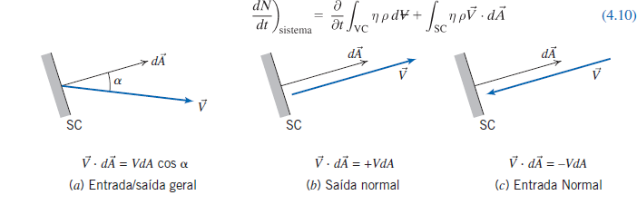
\includegraphics[width=0.7\linewidth]{produtoEscalarVDA.png}
  \caption{Sinais do produto escalar $\vec{V} \cdot d\vec{A}$}
  \label{fig:produtoEscalarVDA}
\end{figure}
A equação da quantidade de movimento é uma equação vetorial e, geralmente, escreveremos as três componentes escalares, como medidas nas coordenadas \textit{xyz} do volume de controle:
\begin{align}
  F_x&=F_S_x+F_B_x=\frac{\partial}{\partial t}\int_{VC}^{ } u\rho\, d\stkout{V} + \int_{SC}^{ } u\rho\vec{V}\cdot\, d\vec{A}\\
  F_y&=F_S_y+F_B_y=\frac{\partial}{\partial t}\int_{VC}^{ } v\rho\, d\stkout{V} + \int_{SC}^{ } v\rho\vec{V}\cdot\, d\vec{A}\\
  F_z&=F_S_z+F_B_z=\frac{\partial}{\partial t}\int_{VC}^{ } w\rho\, d\stkout{V} + \int_{SC}^{ } w\rho\vec{V}\cdot\, d\vec{A}
\end{align}
ou para escoamento uniforme:
\begin{align}
  F_x&=F_S_x+F_B_x=\frac{\partial}{\partial t}\int_{VC}^{ } u\rho\, d\stkout{V} + \sum\nolimits_{SC}^{ } u\rho\vec{V}\cdot \vec{A}\\
  F_y&=F_S_y+F_B_y=\frac{\partial}{\partial t}\int_{VC}^{ } v\rho\, d\stkout{V} + \sum\nolimits_{SC}^{ } v\rho\vec{V}\cdot \vec{A}\\
  F_z&=F_S_z+F_B_z=\frac{\partial}{\partial t}\int_{VC}^{ } w\rho\, d\stkout{V} + \sum\nolimits_{SC}^{ } w\rho\vec{V}\cdot \vec{A}
\end{align}
Notar que, conforme foi mostrado para a equação da conservação da massa \ref{eq:conservacaoMassaEscoamentoCompressivelRegimePermanente}, para escoamento em regime permanente, o primeiro termo após a igualdade é zero pois não há variação das propriedades do fluido.
\end{document}
